% 第 5 章 Constraining Ports and Nets
\bichapter{约束端口与网线}{Constraining Ports and Nets}
\label{chap:ports}

时序分析与时序优化依赖于描述 block 中端口与网线特性的约束。本章说明这些约束及相关任务：
\begin{itemize}
  \item 指定输入端口与 inout 端口的驱动特性
  \item 为端口设置驱动单元
  \item 设置驱动电阻
  \item 设置输入转换时间
  \item 从端口去掉驱动特性
  \item 指定端口负载电容
  \item 理想网络简介
  \item 理想网络属性的传播
  \item 创建与删除理想网络
  \item 报告理想网络
  \item 检索理想对象
  \item 设置理想 latency 与理想转换时间
  \item 时序分析中忽略网线延迟
\end{itemize}

\section{指定输入端口与 inout 端口的驱动特性}
\subsection*{Specifying Drive Characteristics at Input and Inout Ports}

要约束输入或 inout 端口，应为它指定驱动电阻与输入转换时间，方法有两种：
\begin{itemize}
  \item 用 \cmd{set\_driving\_cell} 指定外部驱动单元。工具据此计算驱动电阻与输入转换时间。端口还会继承驱动单元的其他特性，例如设计规则约束。这是更准确的驱动特性表示。
  \item 用 \cmd{set\_drive} 与 \cmd{set\_input\_transition} 直接指定驱动电阻与输入转换时间。这是较不准确的表示。
\end{itemize}

若两种方法都用，由 \cmd{set\_driving\_cell} 所指定驱动单元导出的驱动电阻与输入转换时间，会替换 \cmd{set\_drive} 与 \cmd{set\_input\_transition} 指定的值。

用 \cmd{report\_ports -drive} 报告端口上的驱动单元，或驱动电阻与输入转换时间。

\section{为端口设置驱动单元}
\subsection*{Setting a Drive Driving Cell for Ports}

可以用 \cmd{set\_driving\_cell} 建模端口的外部驱动特性，从而约束输入或 inout 端口。工具使用驱动单元的时序弧来计算被约束端口的驱动特性。

必须指定：
\begin{itemize}
  \item 正在约束的端口。
  \item 用 \opt{-lib\_cell} 指定外部驱动器的库单元。使用该选项时，还要用 \opt{-library} 给出取得该单元的库名。若不指定库，工具从找到的第一个含有匹配单元的参考库中取得该单元。
\end{itemize}

还可以指定：
\begin{itemize}
  \item 用 \opt{-rise} 与 \opt{-fall} 为上升与下降转换分别指定驱动单元。默认同一个驱动单元同时用于两者。
  \item 用 \opt{-min} 与 \opt{-max} 为 early 与 late 分析分别指定驱动单元。默认同时用于两者。
  \item 用 \opt{-pin} 指定用来驱动端口的库单元输出引脚。若所指定的库单元有多个输出引脚且未使用该选项，工具随机挑选一个输出引脚来驱动被约束端口。
  \item 用 \opt{-from\_pin} 指定驱动单元的输入引脚，以选择用于计算驱动特性的时序弧。若不使用该选项，工具随机挑选驱动单元的一个输入引脚。
  \item 用 \opt{-input\_transition\_rise} 与 \opt{-input\_transition\_fall} 指定驱动单元输入端的上升与下降转换时间，用于计算驱动特性。默认驱动单元输入端的转换时间为零。
  \item 用 \opt{-dont\_scale} 要求工具不要按 block 的工作条件缩放驱动特性。默认会按工作条件缩放。
  \item 用 \opt{-no\_design\_rule} 要求不要把驱动单元的设计规则加到被约束端口上。默认会施加这些设计规则。
  \item 用 \opt{-multiply\_by} 给出一个乘数，乘到为被约束端口计算出的转换时间上。
\end{itemize}

对多 scenario 设计，所指定的驱动单元默认只作用于当前 scenario。还可以：
\begin{itemize}
  \item 用 \opt{-modes} 指定某些 mode 的全部 scenario。
  \item 用 \opt{-corners} 指定某些 corner 与当前 mode 的全部 scenario。
  \item 同时用 \opt{-modes} 与 \opt{-corners}。
  \item 用 \opt{-scenarios} 指定具体 scenario。使用该选项时不能再用 \opt{-modes} 或 \opt{-corners}。
\end{itemize}

下例用类型为 \cmd{AND2} 的库单元约束端口 \cmd{I2}，选择从其输入引脚 \cmd{A} 出发的时序弧，并把该输入引脚的上升与下降转换时间指定为 0.5：
\begin{lstlisting}
icc2_shell> set_driving_cell [get_ports I2] \
    -lib_cell AND2 -from_pin A \
    -input_transition_rise 0.5 -input_transition_fall 0.5
\end{lstlisting}

\begin{figure}[htbp]
  \centering
  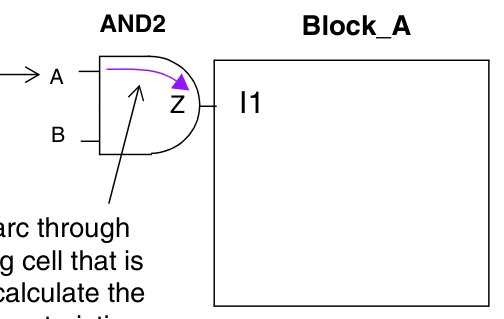
\includegraphics[width=0.72\textwidth]{fig-5-1.png}
  \caption{为驱动单元指定输入引脚与输入转换时间}
  \label{fig:drv-cell}
\end{figure}

\section{设置驱动电阻}
\subsection*{Setting Drive Resistance}

可以用 \cmd{set\_drive} 把外部驱动强度建模为一个电阻值，从而约束输入或 inout 端口。外部驱动器被建模为电源与该电阻串联。

必须指定正在约束的端口以及驱动电阻。还可以：
\begin{itemize}
  \item 用 \opt{-rise} 与 \opt{-fall} 为上升与下降分别指定驱动电阻。默认同时作用于两者。
  \item 用 \opt{-min} 与 \opt{-max} 为 early 与 late 分析分别指定驱动电阻。默认同时作用于两者。
\end{itemize}

对多 scenario 设计，驱动电阻默认只作用于当前 scenario。范围选项与 \cmd{set\_driving\_cell} 相同：\opt{-modes}、\opt{-corners}、两者同时，或 \opt{-scenarios}。

下例把端口 \cmd{A}、\cmd{B}、\cmd{C} 的上升与下降驱动电阻设为 2.0：
\begin{lstlisting}
icc2_shell> set_drive 2.0 {A B C}
\end{lstlisting}

\cmd{set\_driving\_cell} 是指定输入或 inout 端口驱动特性的更准确方法。若无法指定驱动单元，再用 \cmd{set\_drive} 与 \cmd{set\_input\_transition} 指定外部驱动特性。

\section{设置输入转换时间}
\subsection*{Setting an Input Transition Time}

用 \cmd{set\_input\_transition} 为输入或 inout 端口指定固定转换时间。端口的单元延迟为零。工具只在计算该端口所驱动逻辑的延迟时使用这个转换时间。

必须指定正在约束的端口以及输入转换时间。还可以：
\begin{itemize}
  \item 用 \opt{-rise} 与 \opt{-fall} 分别指定上升与下降输入转换时间。默认同时作用于两者。
  \item 用 \opt{-min} 与 \opt{-max} 分别指定 early 与 late 分析的输入转换时间。默认同时作用于两者。
  \item 用 \opt{-clock} 把输入转换时间相对某个时钟来指定。默认使用该时钟的上升沿。要使用下降沿，再加 \opt{-clock\_fall}。
\end{itemize}

对多 scenario 设计，输入转换时间默认只作用于当前 scenario。范围选项与前面相同。

下例把端口 \cmd{A}、\cmd{B}、\cmd{C} 的上升与下降输入转换时间设为 0.5：
\begin{lstlisting}
icc2_shell> set_input_transition 0.5 {A B C}
\end{lstlisting}

\section{从端口去掉驱动特性}
\subsection*{Removing Drive Characteristics From Ports}

表~\ref{tab:rm-drive} 中的命令从端口上去掉驱动信息。

\begin{table}[htbp]
\centering
\caption{去掉驱动信息的命令}
\label{tab:rm-drive}
\begin{tabularx}{\textwidth}{@{}X l@{}}
\toprule
要去掉的内容 & 使用的命令 \\
\midrule
一组端口上的驱动单元信息 & \cmd{remove\_driving\_cell} \\
驱动电阻 & \cmd{set\_drive 0.0} \\
输入转换时间 & \cmd{set\_input\_transition 0.0} \\
驱动数据以及全部用户指定数据，例如时钟、输入与输出延迟 & \cmd{reset\_design} \\
\bottomrule
\end{tabularx}
\end{table}

\section{指定端口负载电容}
\subsection*{Specifying Port Load Capacitance}

要准确做时序分析，工具需要连接到顶层端口的网线的外部负载电容，包括引脚电容与连线电容。可以用 \cmd{set\_load} 在端口上显式指定负载电容。

必须指定正在约束的端口以及电容值。还可以：
\begin{itemize}
  \item 用 \opt{-rise} 与 \opt{-fall} 分别为上升与下降指定电容。默认同时作用于两者。
  \item 用 \opt{-min} 与 \opt{-max} 分别为 early 与 late 分析指定电容。默认同时作用于两者。
  \item 用 \opt{-wire\_load} 把电容当作线负载；或同时用 \opt{-wire\_load} 与 \opt{-pin\_load}，既当作线负载也当作引脚负载。默认把电容当作引脚负载。
\end{itemize}

下例把全部输入上的电容设为 3.5，全部输出上的电容设为 5：
\begin{lstlisting}
icc2_shell> set_load 3.5 [all_inputs]
icc2_shell> set_load 5 [all_outputs]
\end{lstlisting}

\section{理想网络简介}
\subsection*{Introduction to Ideal Networks}

理想网络（ideal network）是一组免于时序更新、时序优化与 DRC 修复的单元、网线与引脚。理想网络中的对象忽略最大电容与转换时间设计规则。因此运行时间与时序优化都会改善。此外，优化期间工具不会去掉理想网络的源端口或叶级引脚。

例如，若把打算单独综合的某些高扇出网（如 scan-enable 与 reset）标为理想网，就可以避免优化期间不必要的 retiming 和不希望的设计改动，从而缩短运行时间。

指定理想网络的源端口或叶级引脚后，该源传递扇出中的网线、单元与引脚都被当作理想对象。理想对象具有下列性质：
\begin{itemize}
  \item 被标为 don't touch。
  \item 不受时序更新、延迟优化或 DRC 修复影响。
  \item 被赋予理想时序属性：理想 latency、理想转换时间，以及为零的理想电容。可用 \cmd{set\_ideal\_latency} 与 \cmd{set\_ideal\_transition} 分别修改 latency 与转换时间。
\end{itemize}

包含或驱动该源的单元会被设置 \cmd{size\_only} 属性。这保证 compile 期间理想网络的源不会丢失。

\section{理想网络属性的传播}
\subsection*{Propagation of the Ideal Network Property}

指定理想网络的源对象后，源对象传递扇出中的全部网线、单元与引脚都被当作理想对象。当前设计的任意输入端口或内部引脚都可以作为源对象，但层次边界上的引脚除外。

工具按一定传播规则，自动把理想网络属性扩散到源对象传递扇出中的网线、单元与引脚，并在到达下列位置时停止：
\begin{itemize}
  \item 时序单元。
  \item 不再有前向时序弧的点，例如输出端口或被禁用的时序弧。
  \item 不是理想对象的对象。
\end{itemize}

工具把下列对象视为理想对象：
\begin{itemize}
  \item 满足下列之一的引脚：出现在 \cmd{set\_ideal\_network} 的对象列表中；其单元为理想单元的驱动引脚；连接到理想网的负载引脚。
  \item 全部驱动引脚都是理想引脚的网线。
  \item 满足下列之一的组合单元：全部输入引脚都是理想的；一个输入引脚连接到常数网，且其余输入引脚都是理想的。带有 case analysis 属性的对象不当作常数。
\end{itemize}

若理想网络与时钟网络重叠，时钟时序信息（包括时钟 latency 与转换时间）覆盖重叠网络中时钟部分的理想时序。

对图~\ref{fig:ideal-net} 中的电路，假定把引脚 \cmd{U1/Z} 指定为理想网络的源。工具沿 \cmd{U1/Z} 传递扇出中的网线、单元与引脚传播理想网络属性，并停在名为 \cmd{REG1} 的时序单元处。工具还把 \cmd{dont\_touch} 属性传播到这些网线、单元与引脚，并在理想网络源的驱动器（单元 \cmd{IV1}）上设置 \cmd{size\_only}。

\begin{figure}[htbp]
  \centering
  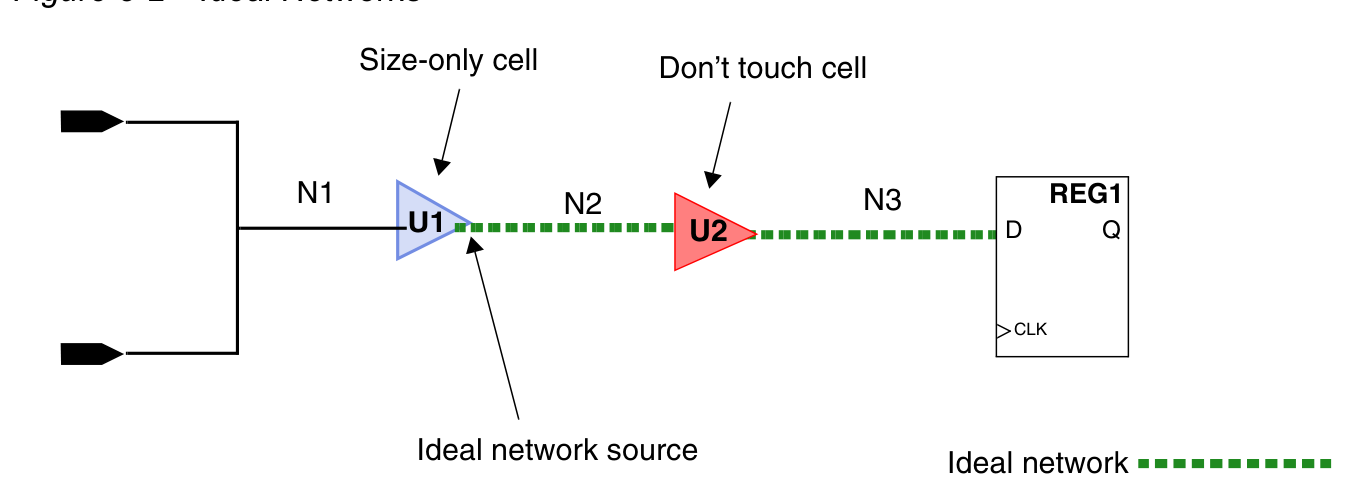
\includegraphics[width=0.9\textwidth]{fig-5-2.png}
  \caption{理想网络}
  \label{fig:ideal-net}
\end{figure}

\begin{figure}[htbp]
  \centering
  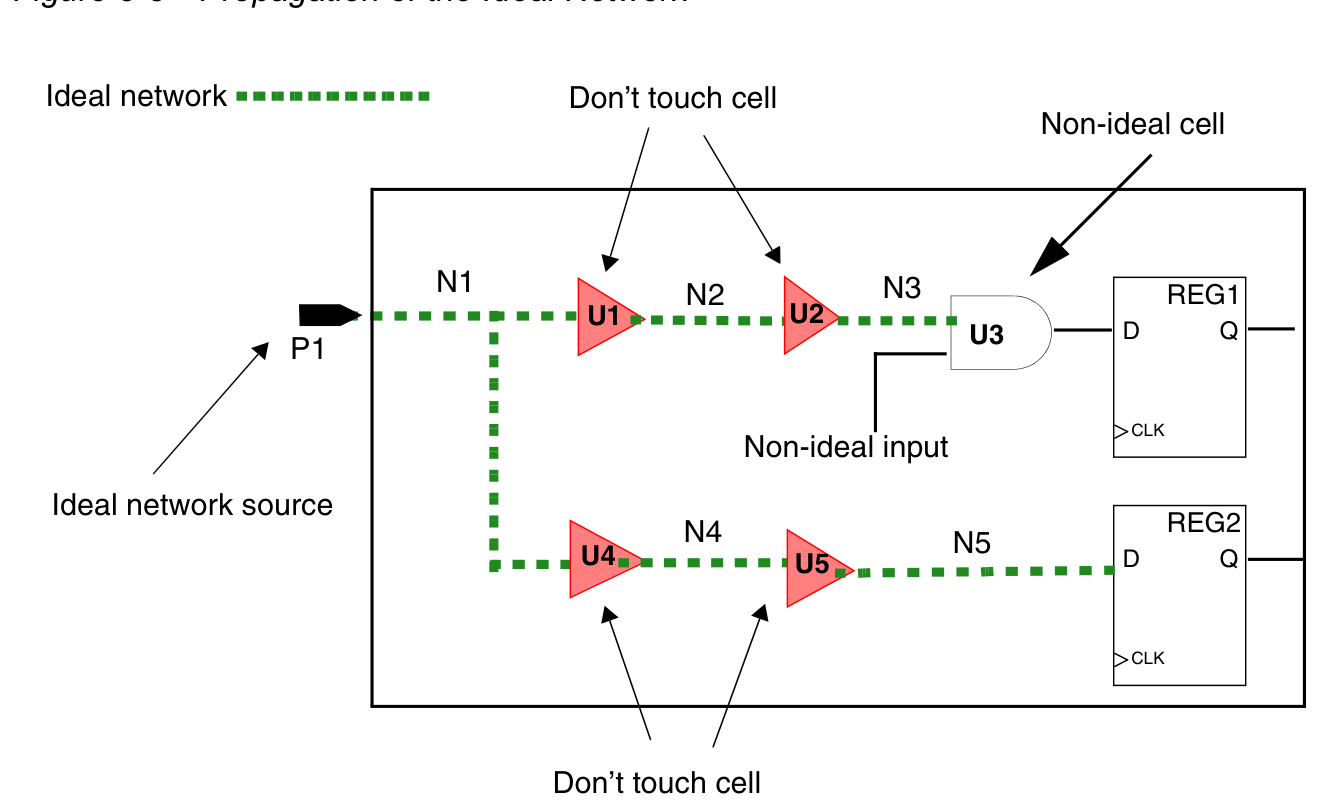
\includegraphics[width=0.9\textwidth]{fig-5-3.png}
  \caption{理想网络属性的传播}
  \label{fig:ideal-prop}
\end{figure}

\section{创建与删除理想网络}
\subsection*{Creating and Removing Ideal Networks}

用 \cmd{set\_ideal\_network} 创建理想网络。必须指定一组端口、引脚或网线作为理想网络的源。若指定的是网线，则该网的全局驱动引脚或端口被标为理想网络源。也就是说，理想网络属性加到所指定网线的全局驱动引脚或端口上。这样即使该网在优化中被去掉，理想网络属性也不会丢失。

用 \opt{-no\_propagate} 阻止理想网络穿过逻辑门继续传播。

下列命令把端口 \cmd{P1} 指定为理想网络的源：
\begin{lstlisting}
icc2_shell> set_ideal_network [get_ports P1]
\end{lstlisting}

用 \cmd{remove\_ideal\_network} 去掉理想网络设置，并把理想网络中的单元、网线与引脚恢复为非理想状态。

\section{报告理想网络}
\subsection*{Reporting Ideal Networks}

可用下列命令取得理想网络的更多信息：
\begin{itemize}
  \item \cmd{remove\_ideal\_network}：把理想网络中的单元、网线与引脚恢复到最初的非理想状态。
  \item \cmd{report\_attributes}：报告与单元、网线、引脚关联的属性。若用它报告理想网上的属性，会报告由 \cmd{set\_ideal\_network -no\_propagate} 设置的属性。
  \item \cmd{report\_nets}：报告网线信息；理想网以 ``I'' 标出。
\end{itemize}

\cmd{report\_timing}、\cmd{report\_cells} 与 \cmd{report\_nets} 会指出传播到理想网络非源对象上的理想网络属性，以及网络的源端口与源引脚。而 \cmd{report\_attributes} 与 \cmd{get\_attribute} 只对网络的源端口与源引脚显示理想网络属性，不显示已传播的属性。

\section{检索理想对象}
\subsection*{Retrieving Ideal Objects}

用下列命令检索理想对象：
\begin{itemize}
  \item \cmd{get\_nets -filter "ideal\_net == true"}：返回由 \cmd{set\_ideal\_network -no\_propagate} 设置的理想网。
  \item \cmd{get\_pins -filter "ideal\_network\_source == true"}：返回作为理想网络源的引脚。若再加过滤条件 \cmd{ideal\_network\_options == 1}，则只返回由 \cmd{set\_ideal\_network -no\_propagate} 设置的理想网络源引脚。
  \item \cmd{get\_ports -filter "ideal\_network\_source == true"}：返回作为理想网络源的端口。过滤条件 \cmd{ideal\_network\_options == 1} 的含义与引脚相同。
\end{itemize}

\section{设置理想 latency 与理想转换时间}
\subsection*{Setting Ideal Latency and Ideal Transition Time}

理想网络的默认 latency 与转换时间都是零。可用下列命令覆盖默认值：
\begin{itemize}
  \item \cmd{set\_ideal\_latency}
  \item \cmd{set\_ideal\_transition}
\end{itemize}

\begin{noteBox}
执行这两条命令中的任意一条时，理想网络的时序都会更新。
\end{noteBox}

这两条命令可以加在理想网或理想网络的源引脚上，也可以加在理想网络的任意非源引脚上。所指定的值覆盖库单元值或网线延迟值。对理想网络，理想 latency 与转换时间从源引脚传播到网络边界引脚。

理想网络中任意一点的总理想 latency，等于源引脚理想 latency 加上沿路径到达该点的各叶单元引脚理想 latency 之和。各源引脚与叶单元引脚上指定的理想转换时间彼此独立、不累积。未指定的输入引脚，其转换时间取最近一个已指定理想转换时间的引脚的值。该规则同样适用于边界引脚。

\cmd{set\_input\_delay} 适用于理想网络。该延迟被当作片外 latency 或 source latency。

用下列命令去掉理想 latency 与理想转换时间：
\begin{itemize}
  \item \cmd{remove\_ideal\_latency}
  \item \cmd{remove\_ideal\_transition}
\end{itemize}

\section{时序分析中忽略网线延迟}
\subsection*{Ignoring Net Delays During Timing Analysis}

默认情况下，IC Compiler II 在时序分析中同时考虑网线延迟与单元延迟。若要忽略网线延迟、只考虑单元延迟，把应用选项 \appopt{time.delay\_calculation\_style} 设为 \cmd{zero\_interconnect}，以启用零互连延迟计算。要把延迟计算风格恢复为默认，把该应用选项设为 \cmd{auto}。
